
\documentclass[a4paper, 10pt, twoside]{article}

\usepackage[top=1in, bottom=1in, left=1in, right=1in]{geometry}
\usepackage[utf8]{inputenc}
\usepackage[spanish, es-ucroman, es-noquoting]{babel}
\usepackage{setspace}
\usepackage{fancyhdr}
\usepackage{lastpage}
\usepackage{amsmath}
\usepackage{amsfonts}
\usepackage{amsthm}
\usepackage{verbatim}
\usepackage{fancyvrb}
\usepackage{graphicx}
\usepackage{float}
\usepackage{enumitem} % Provee macro \setlist
\usepackage{tabularx}
\usepackage{multirow}
\usepackage{hyperref}
\usepackage{xspace}
\usepackage{ulem} % Provee macro \uwave
\usepackage[toc, page]{appendix}


%%%%%%%%%% Constantes - Inicio %%%%%%%%%%
\newcommand{\titulo}{Trabajo Práctico 1}
\newcommand{\materia}{Bases de Datos}
\newcommand{\integrantes}{Russo · Russo · Russo · Russo}
\newcommand{\cuatrimestre}{Primer Cuatrimestre de 2016}
%%%%%%%%%% Constantes - Fin %%%%%%%%%%


%%%%%%%%%% Configuración de Fancyhdr - Inicio %%%%%%%%%%
\pagestyle{fancy}
\thispagestyle{fancy}
\lhead{\titulo · \materia}
\rhead{\integrantes}
\renewcommand{\footrulewidth}{0.4pt}
\cfoot{\thepage /\pageref{LastPage}}

\fancypagestyle{caratula} {
   \fancyhf{}
   \cfoot{\thepage /\pageref{LastPage}}
   \renewcommand{\headrulewidth}{0pt}
   \renewcommand{\footrulewidth}{0pt}
}
%%%%%%%%%% Configuración de Fancyhdr - Fin %%%%%%%%%%


%%%%%%%%%% Miscelánea - Inicio %%%%%%%%%%
% Evita que el documento se estire verticalmente para ocupar el espacio vacío
% en cada página.
\raggedbottom

% Separación entre párrafos.
\setlength{\parskip}{0.5em}

% Separación entre elementos de listas.
\setlist{itemsep=0.5em}

% Asigna la traducción de la palabra 'Appendices'.
\renewcommand{\appendixtocname}{Apéndices}
\renewcommand{\appendixpagename}{Apéndices}
%%%%%%%%%% Miscelánea - Fin %%%%%%%%%%


%%%%%%%%%% Macros para el modelo relacional - Inicio %%%%%%%%%%
\newcommand{\relacion}[3]{
  \noindent
  \textbf{#1}(\ignorespaces#2\unskip) \\
  #3
  \vspace{0.5em}
}
\newcommand{\pk}[1]{%
  \underline{#1}%
}
\newcommand{\fk}[1]{%
  \uwave{#1}%
}
\newcommand{\pkfk}[1]{%
  \pk{\fk{#1}}%
}
\newcommand{\clavespkck}[1]{
  PK = CK = \{#1\}
}
\newcommand{\clavespkckfk}[1]{
  PK = CK = FK = \{#1\}
}
\newcommand{\clavesfk}[1]{
  FK = \{#1\}
}
%%%%%%%%%% Macros para el modelo relacional - Fin %%%%%%%%%%

\begin{document}


%%%%%%%%%%%%%%%%%%%%%%%%%%%%%%%%%%%%%%%%%%%%%%%%%%%%%%%%%%%%%%%%%%%%%%%%%%%%%%%
%% Carátula                                                                  %%
%%%%%%%%%%%%%%%%%%%%%%%%%%%%%%%%%%%%%%%%%%%%%%%%%%%%%%%%%%%%%%%%%%%%%%%%%%%%%%%


\thispagestyle{caratula}

\begin{center}


\includegraphics[height=2cm]{DC.png} 
\hfill

\includegraphics[height=2cm]{UBA.jpg} 

\vspace{2cm}

Departamento de Computación,\\
Facultad de Ciencias Exactas y Naturales,\\
Universidad de Buenos Aires

\vspace{4cm}

\begin{Huge}
\titulo
\end{Huge}

\vspace{0.5cm}

\begin{Large}
\materia
\end{Large}

\vspace{1cm}

\cuatrimestre

\vspace{4cm}

\begin{tabular}{|c|c|c|}
\hline
Apellido y Nombre & LU & E-mail\\
\hline
Russo, Christian  & 679/10 & christian.russo8@gmail.com\\
Russo, Christian  & 679/10 & christian.russo8@gmail.com\\
Russo, Christian  & 679/10 & christian.russo8@gmail.com\\
Russo, Christian  & 679/10 & christian.russo8@gmail.com\\
\hline
\end{tabular}

\end{center}

\newpage


%%%%%%%%%%%%%%%%%%%%%%%%%%%%%%%%%%%%%%%%%%%%%%%%%%%%%%%%%%%%%%%%%%%%%%%%%%%%%%%
%% Introducción                                                              %%
%%%%%%%%%%%%%%%%%%%%%%%%%%%%%%%%%%%%%%%%%%%%%%%%%%%%%%%%%%%%%%%%%%%%%%%%%%%%%%%


\section{Introducción}

Presentaremos una soluci\'on para el problema de un \textbf{Mercado Virtual} tomando como gu\'ia el \textbf{Khan El-Khalili} ubicado en El Cairo, Egipto. El problema en cuesti\'on contempla una serie de restricciones sobre como se realizan la combra y venta de productos por internet. Cada publicacion puede tener distintos tipos y ser de distintas formas, haciendo que esto impacte en la facturacion del usuario que publica. Por otro lado se cuenta con un sistema de comentarios y calificaciones.

Utilizaremos las herramientas vistas en la materia, el modelado basado en el Diagrama de Entidad Relaci?on, su MR resultante y la base de datos final que presentaremos en MySQL.

%%%%%%%%%%%%%%%%%%%%%%%%%%%%%%%%%%%%%%%%%%%%%%%%%%%%%%%%%%%%%%%%%%%%%%%%%%%%%%%
%% Diagrama de Entidad Relación                                              %%
%%%%%%%%%%%%%%%%%%%%%%%%%%%%%%%%%%%%%%%%%%%%%%%%%%%%%%%%%%%%%%%%%%%%%%%%%%%%%%%


\section{Diagrama de Entidad Relación}

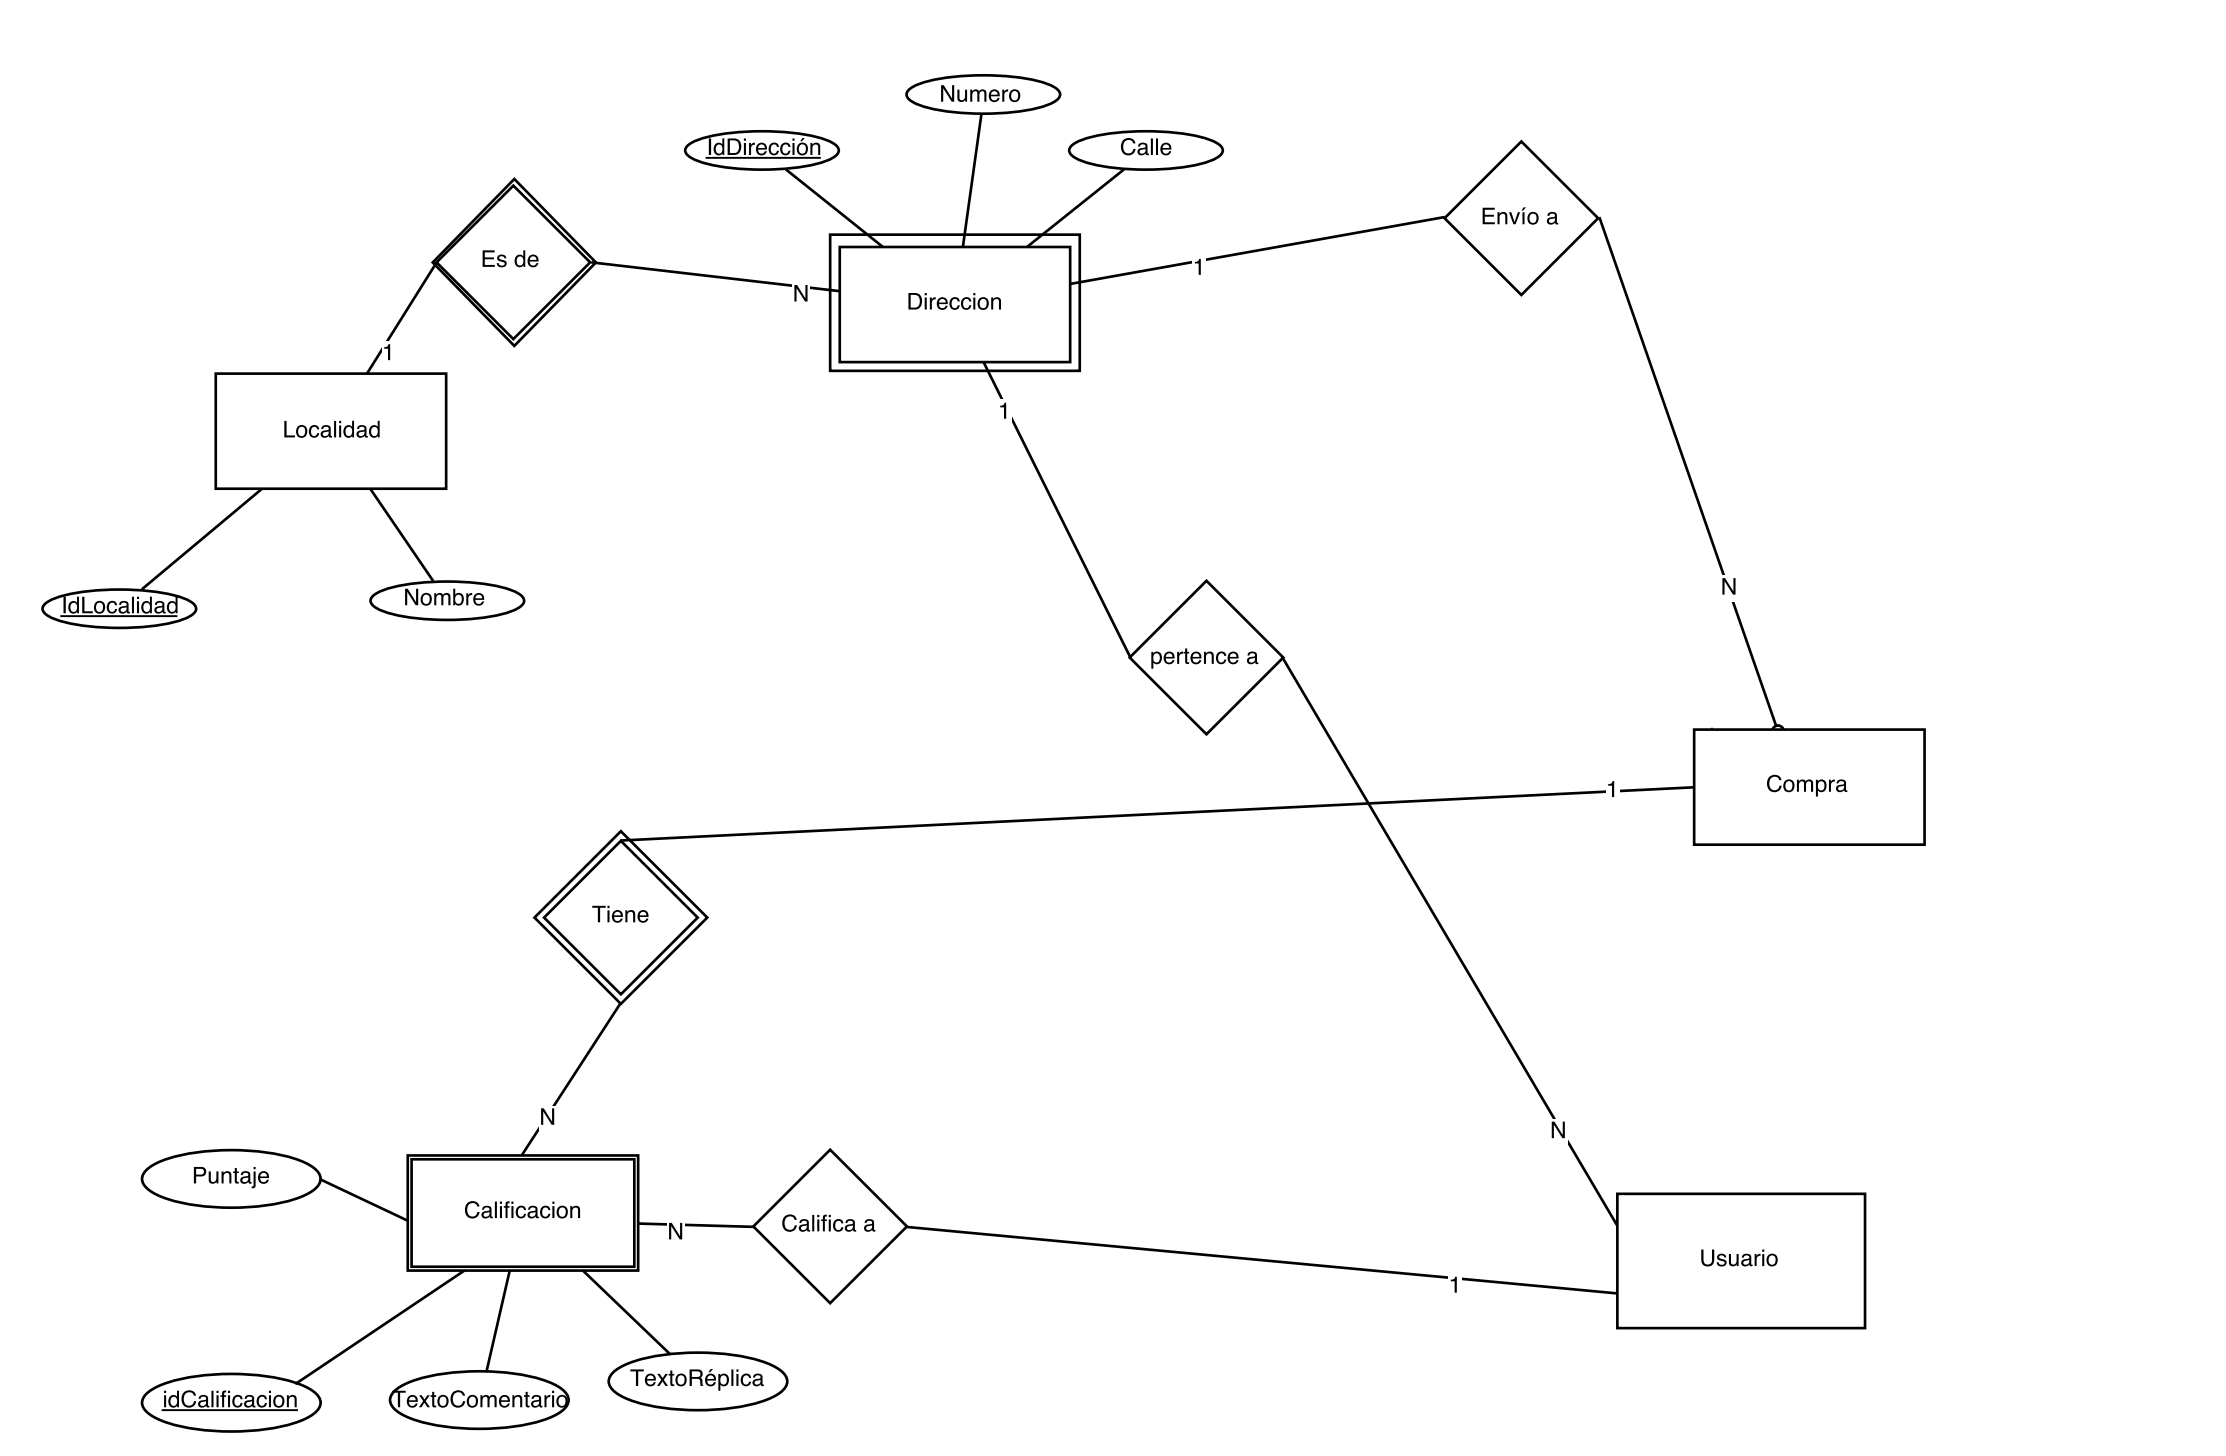
\includegraphics[width=20cm, height=12cm]{der1}
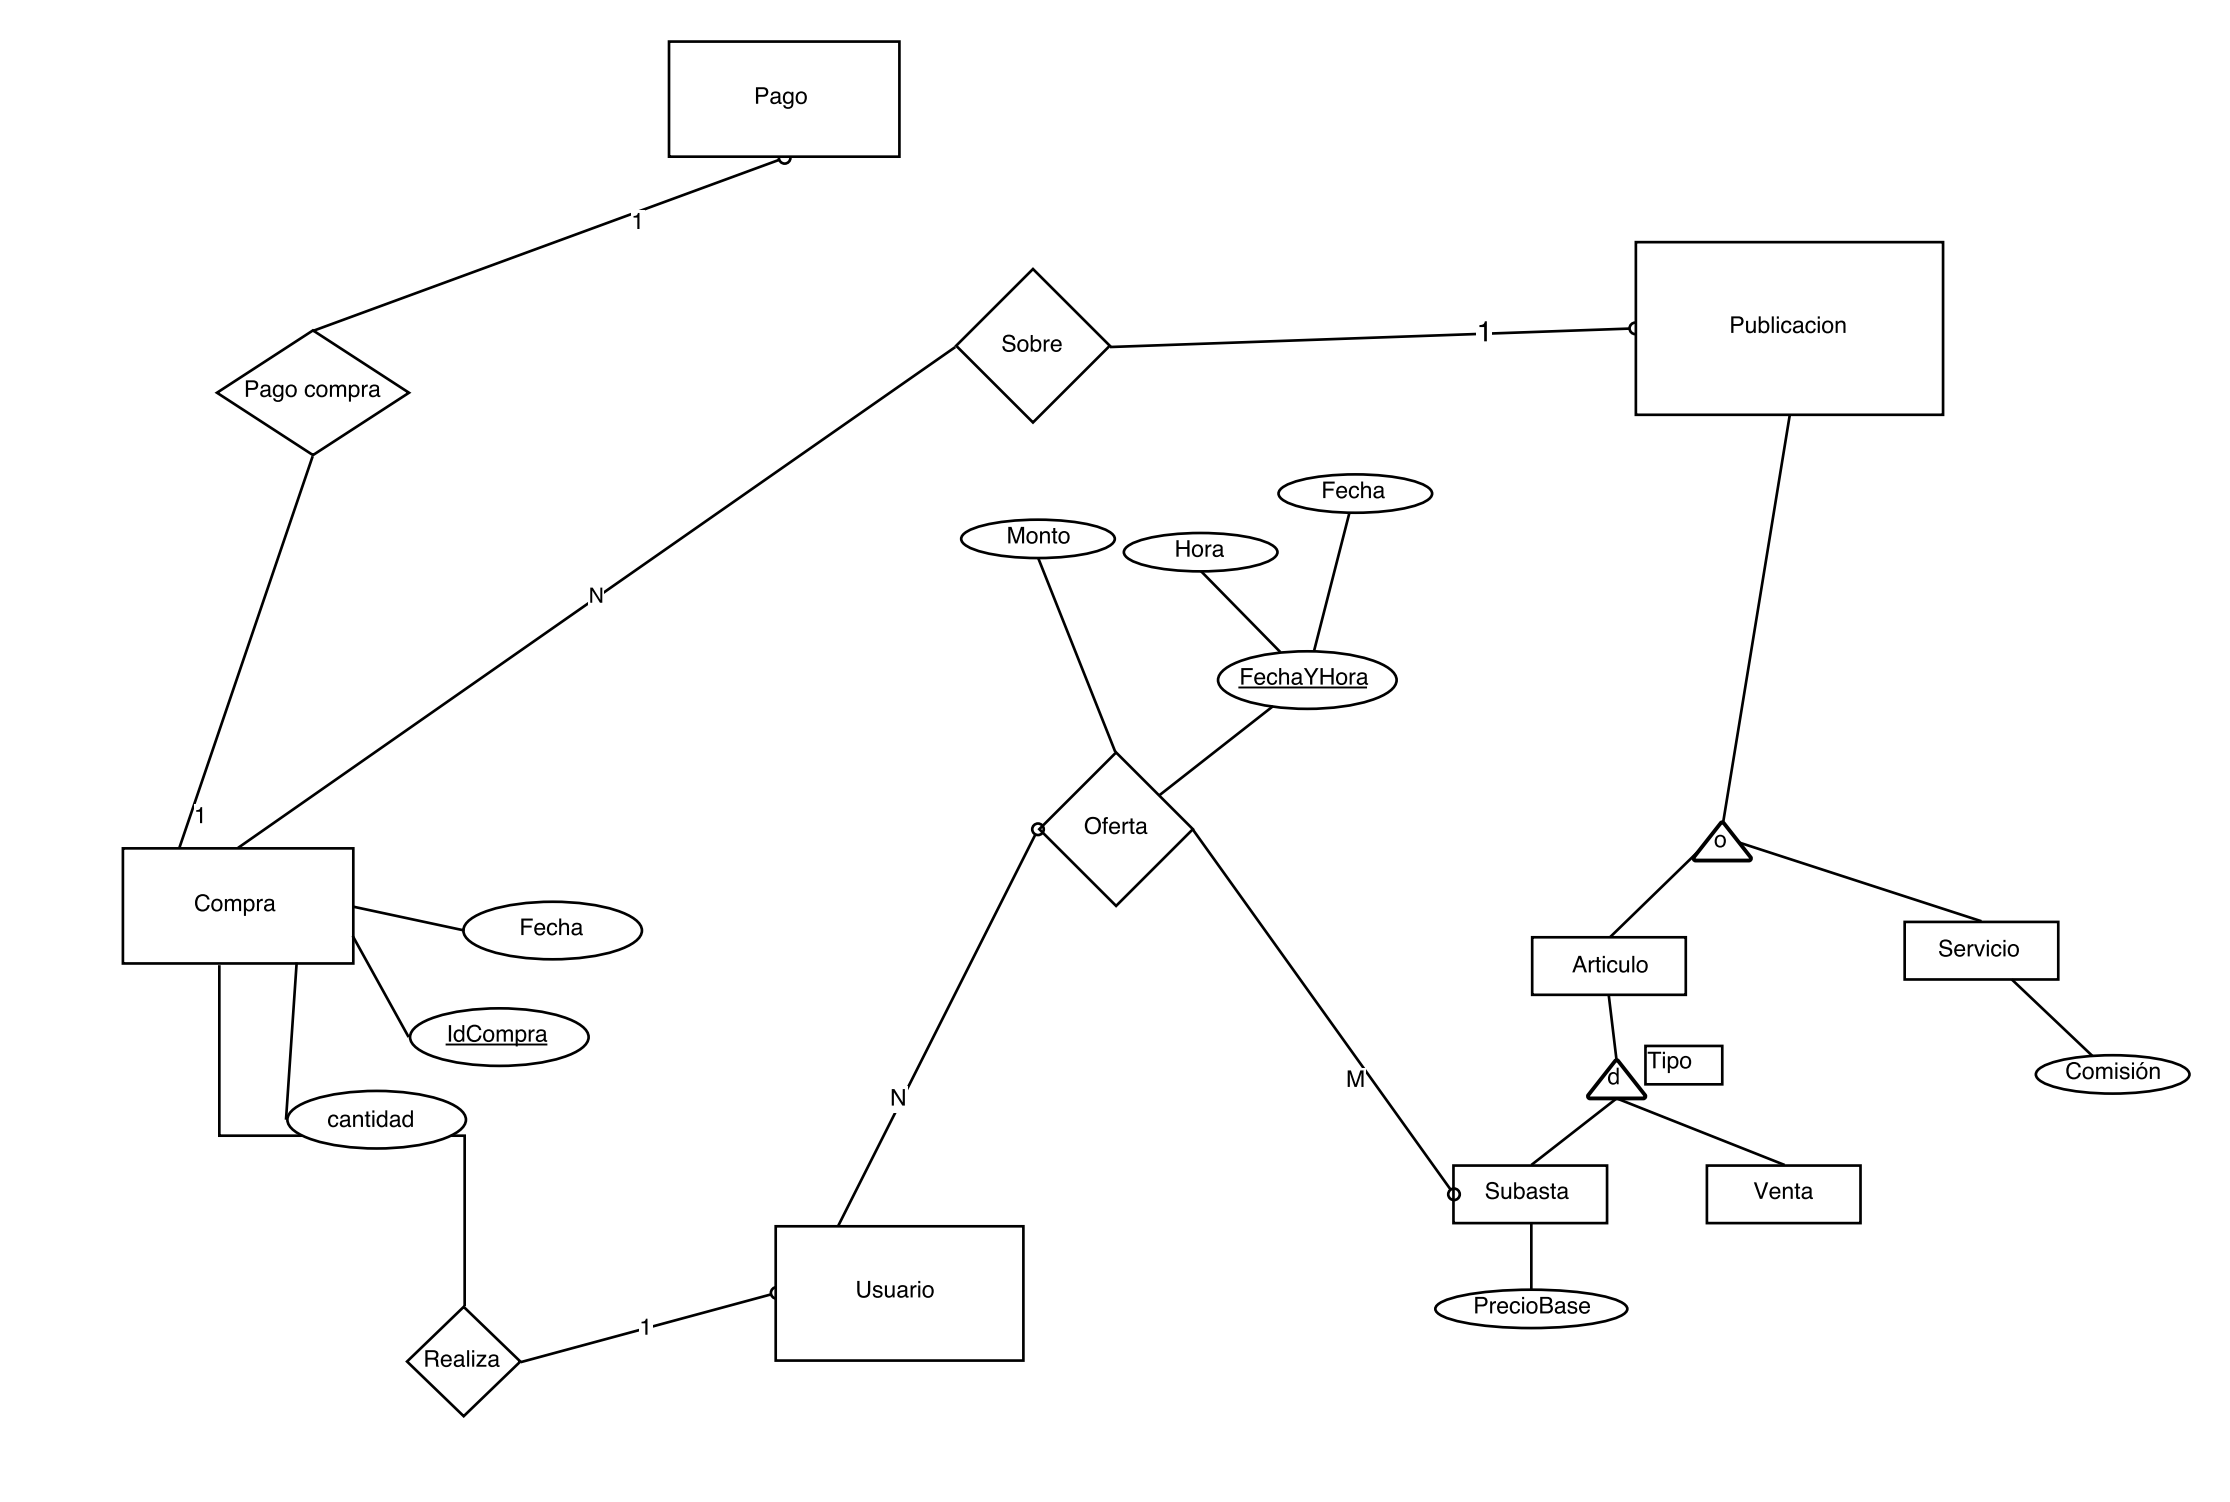
\includegraphics[width=18cm, height=12cm]{der2}
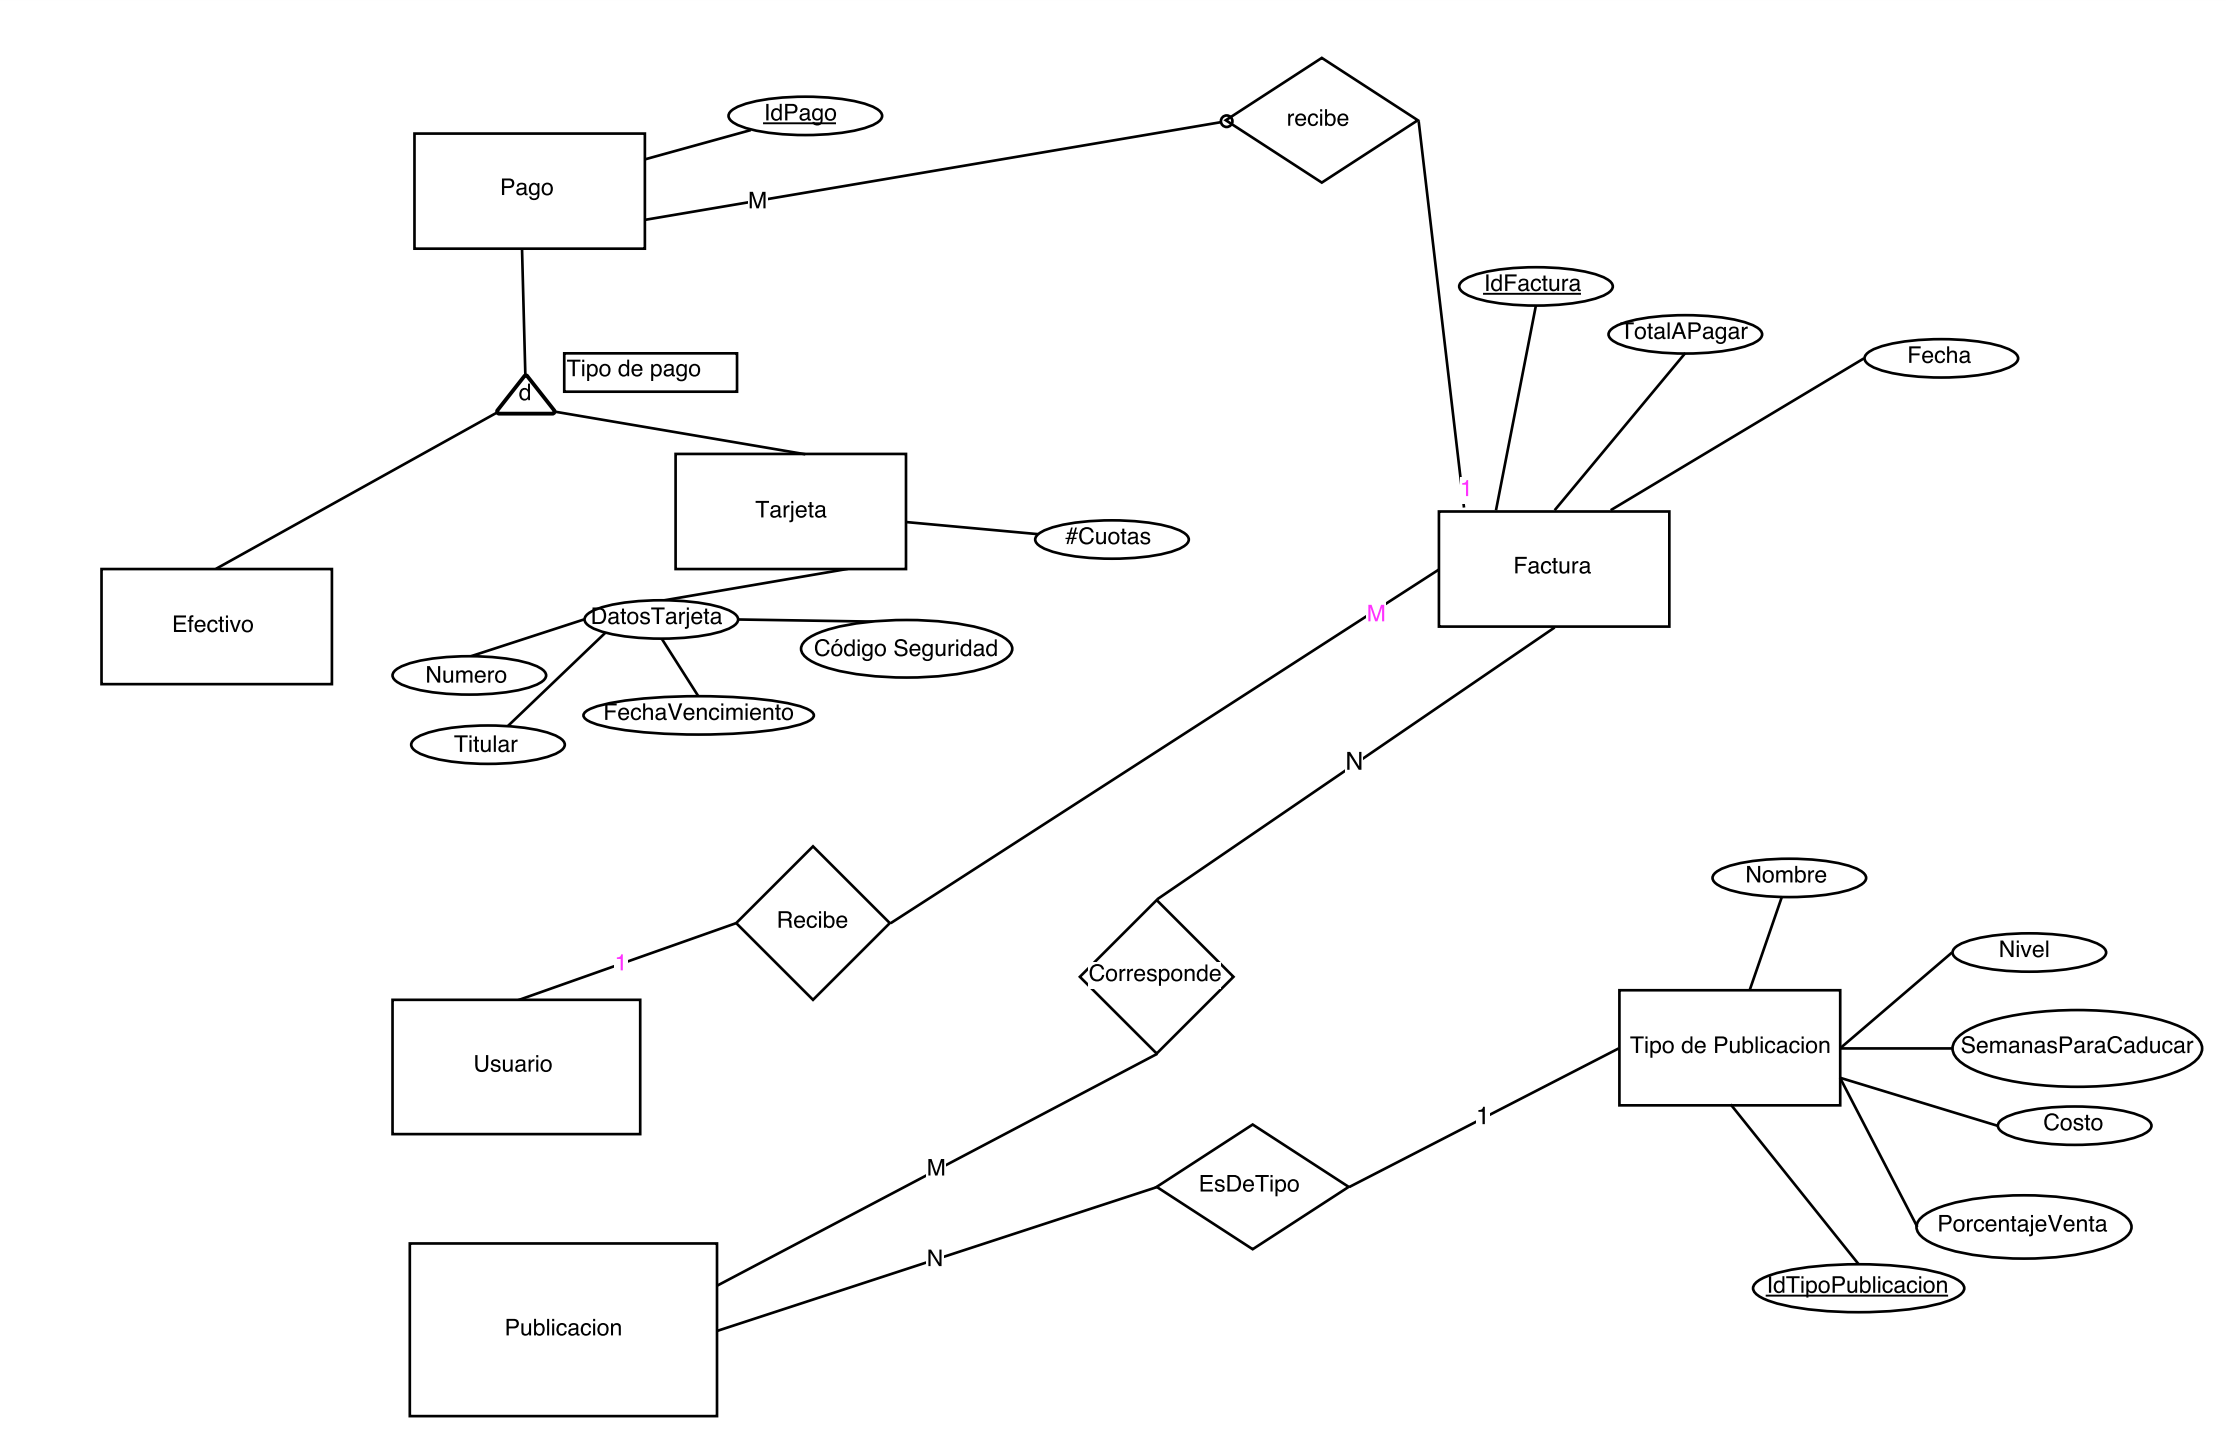
\includegraphics[width=18cm, height=12cm]{der3}
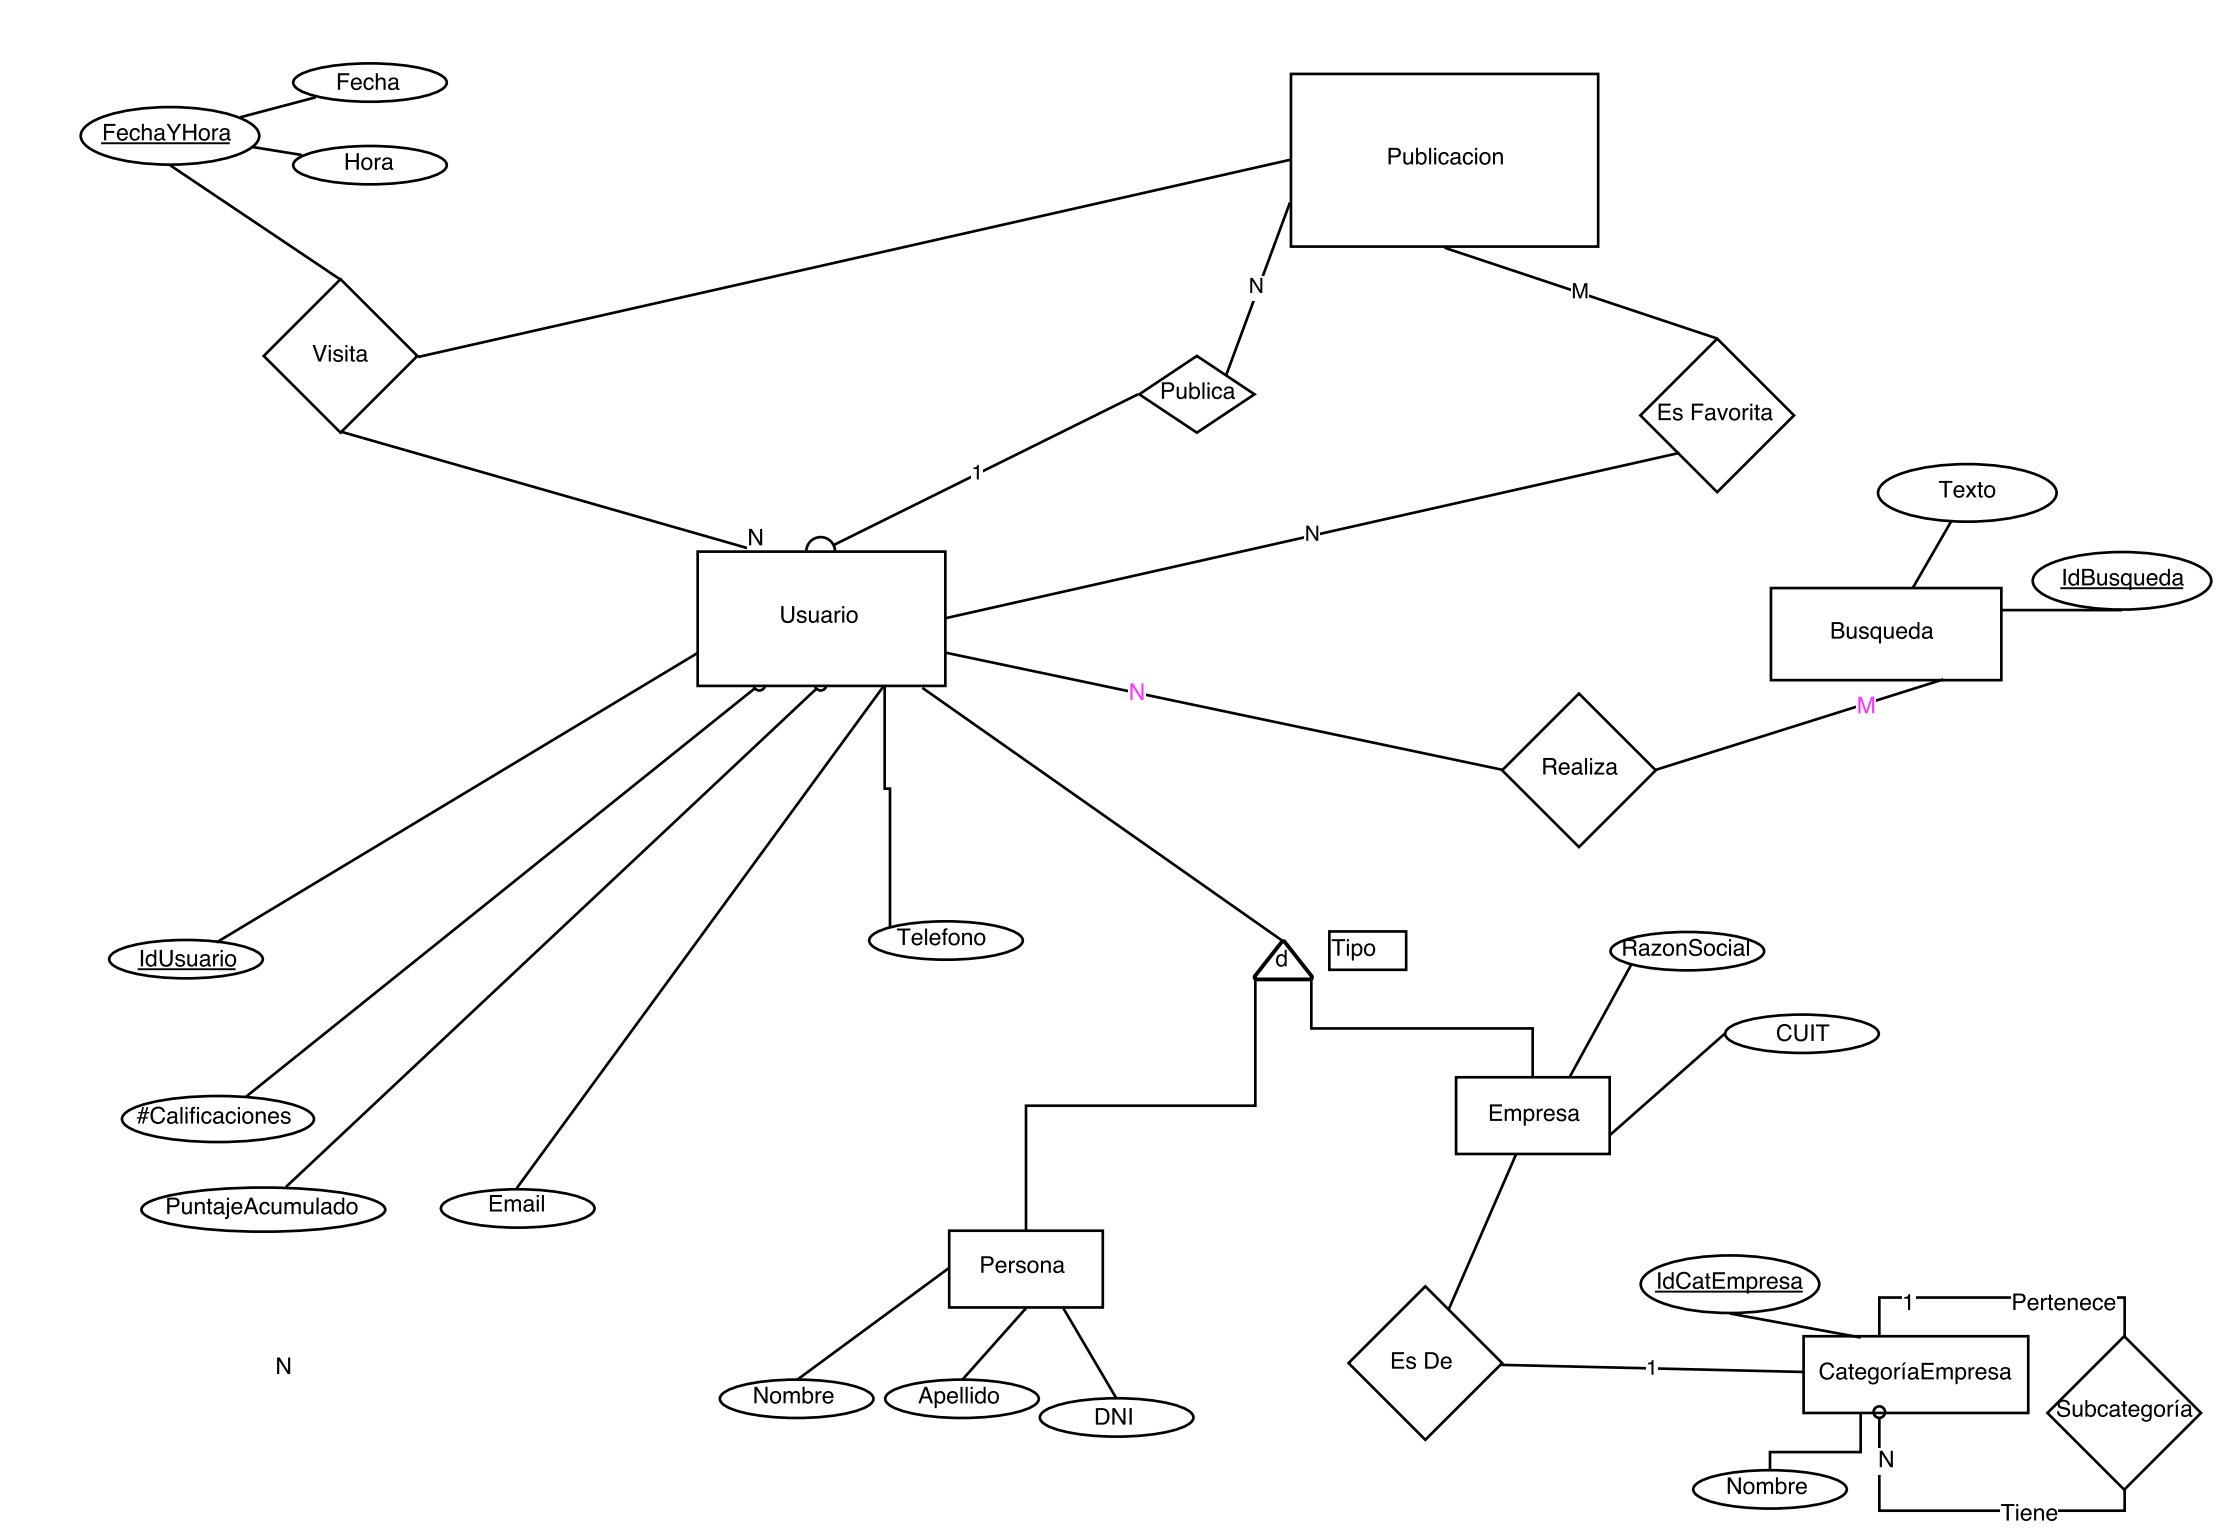
\includegraphics[width=18cm, height=12cm]{der4}
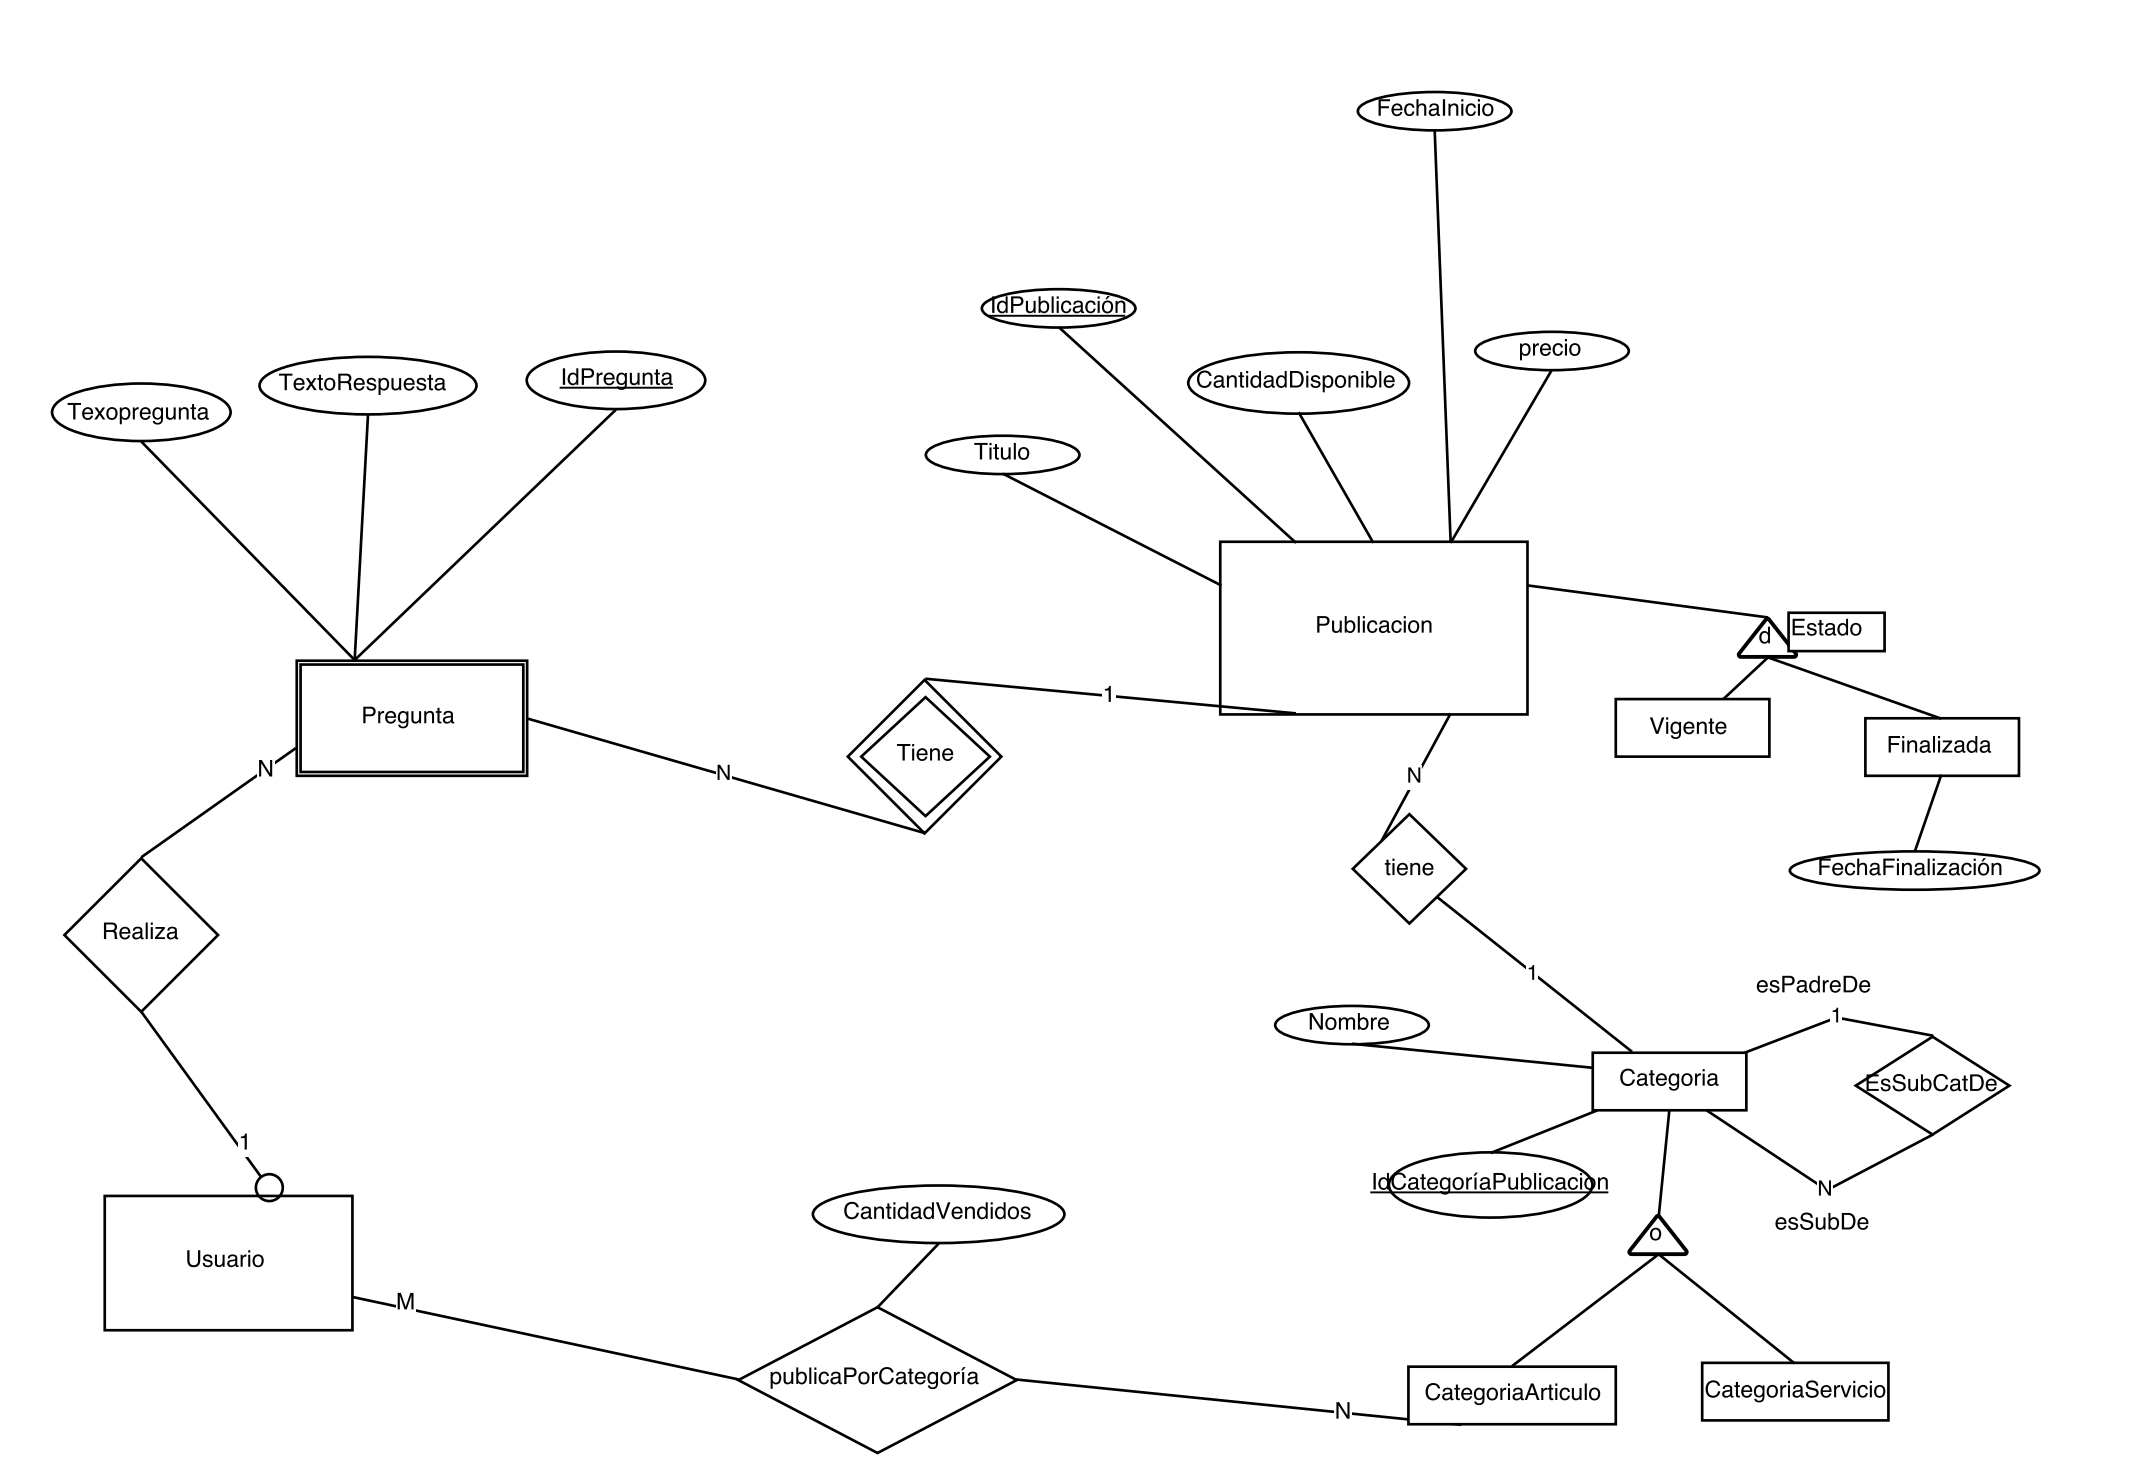
\includegraphics[width=19cm, height=12cm]{der5}

\subsection{Restricciones}

\begin{enumerate}
\item No puede haber dos DNI iguales. 
\item La publicaci\'on del tipo Libre! tiene costo 0.
\item Para cada compraventa existen a lo sumo 2 calificaciones, cada una correspondiente al comprador y vendedor.
\item El nivel de la publicaci\'on es distinto para cada tipo de publicaci\'on.
\item El usuario que compra una publicaci\'on no puede ser el usuario que publica.
\item Si un usuario realiza una respuesta a un comentario, entonces dicho comentario es de una calificaci\'on y la calificaci\'on fue hecha por un usuario que hizo dicha  compra 
\item Las publicaciones del tipo Rub\'iDelOriente aparecen primeras en las b\'usquedas. Luego aparecen en orden de mayor a menor costo de comisi\'on y por \'ultimo las de la categor\'ia Libre!.
\item El costo por mes de Rub\'iDeOriente es Fijo y se pueden hacer 3 publicaciones por mes de este tipo usuario.
\item El costo de las de Oro cobran m\'as porcentaje de la venta como comisi\'on que las de Plata
\item El costo de las de Plata cobran m\'as porcentaje de la venta como comisi\'on que las de Bronce 
\item El monto de una oferta en una subasta debe ser superior en al menos 1 peso a la oferta actual, e inferior al doble de la oferta actual
\item Una calificaci\'on tiene completado el atributo textoR\'eplica, entonces tiene completado el atributo textoComentario
\item El atributo puntaje de calificaci\'on est\'a entre [1, 10].
\item El atributo nombre de la entidad Tipo s\'olo puede ser uno de los siguientes: Rub\'iDeOriente,  Oro,  Plata,  Bronce o Libre! 
\item No se puede realizar una pregunta a una publicaci\'on que est\'a finalizada.
\item El atributo cantidad de la entidad compra siempre es menor o igual al atributo cantidadDisponible de la publicacion.
\item Si el atributo cantidadDisponible de la entidad Publicaci\'on vale 0, entonces la publicaci\'on est\'a finalizada. 
	
\item Dada una oferta, el monto de dicha oferta debe ser mayor en al menos 1 peso a todas las ofertas anteriores (en fecha), y al precioBase de la subasta. Adem\'as dicha oferta no puede superar el doble del precio base.
\item El precio de una publicaci\'on que es de tipo subasta es igual a:
el precioBase de la subasta si no hay una oferta realizada.

\item  Un usuario no puede ofertar en una publicaci\'on finalizada. 
\item  Si un usuario compr\'o una publicaci\'on de tipo subasta, entonces dicho usuario tiene que tener la oferta m\'as alta en dicha publicaci\'on. 
\item El TotalAPagar de la Factura es lo que adeuda el Usuario al sistema en concepto de abonos a Rub\'iDeOriente y/o comisi\'on por las ventas de sus programador. 
\item Un pago o se relaciona con una Publicaci\'on, o se relaciona con una Compra. Nunca con los dos.
\item El atributo CantidadVendidos de la relaci\'on publicaPorCategoria es igual a todas las ventas que realiz\'o ese usuario en esa categor\'ia.
\item El tipo dentro de la tabla Articulo puede ser o venta o subaste 

\end{enumerate}


%%%%%%%%%%%%%%%%%%%%%%%%%%%%%%%%%%%%%%%%%%%%%%%%%%%%%%%%%%%%%%%%%%%%%%%%%%%%%%%
%% Modelo Relacional                                                         %%
%%%%%%%%%%%%%%%%%%%%%%%%%%%%%%%%%%%%%%%%%%%%%%%%%%%%%%%%%%%%%%%%%%%%%%%%%%%%%%%


\section{Modelo Relacional}


\relacion{Persona}{
  \pk{idUsuario},
  nombre,
  apellido,
  DNI
}{
  \clavespkck{idUsuario}
}

\relacion{Empresa}{
  \pk{\fk{idUsuario}},
  RazonSocial.
  CUIT,
  \fk{idCatEmpresa}
}{
  \clavespkck{idUsuario} \\
  \clavesfk{idUsuario, idCatEmpresa}
}

\relacion{CategoriaEmpresa}{
  \pk{idCaEmpresa},
  Nombre.
  \fk{IdCategoriaPadre}
}{
  \clavespkck{idCaEmpresa} \\
  \clavesfk{IdCategoriaPadre}
}


\relacion{Articulo}{
  \pk{\fk{IdPublicacion}},
  tipo
}{
  \clavespkck{IdPublicacion} \\
  \clavesfk{IdPublicacion}
}

\relacion{Subasta}{
  \pk{\fk{IdPublicacion}},
  PrecioBase
}{
  \clavespkck{IdPublicacion} \\
  \clavesfk{IdPublicacion}
}


\relacion{Oferta}{
  \pk{\fk{IdPublicacion,idUsuario}},
  \pk{FechaYHora},
  Monto
}{
  \clavespkck{IdPublicacion,idUsuario,FechaYHora} \\
  \clavesfk{IdPublicacion, idUsuario}
}

\relacion{Venta}{
  \pk{\fk{IdPublicacion}},
}{
  \clavespkck{IdPublicacion} \\
  \clavesfk{IdPublicacion}
}

\relacion{Servicio}{
  \pk{\fk{IdPublicacion}},
  Comision
}{
  \clavespkck{IdPublicacion} \\
  \clavesfk{IdPublicacion}
}

\relacion{Vigente}{
  \pk{\fk{IdPublicacion}}
}{
  \clavespkck{IdPublicacion} \\
  \clavesfk{IdPublicacion}
}

\relacion{Finalizada}{
  \pk{\fk{IdPublicacion}},
  FechaFinalizacion
}{
  \clavespkck{IdPublicacion} \\
  \clavesfk{IdPublicacion}
}

\relacion{Categoria}{
  \pk{IdCategoriaPublicacion},
  Nombre,
  \fk{IdCategoriaPadre}
}{
  \clavespkck{IdCategoriaPublicacion} \\
  \clavesfk{IdCategoriaPadre}
}

\relacion{CategoriaArticulo}{
  \pk{\fk{IdCategoriaPublicacion}}
}{
  \clavespkck{IdCategoriaPublicacion} \\
  \clavesfk{IdCategoriaPublicacion}
}

\relacion{publicaPorCategoria}{
  \pk{\fk{IdCategoriaPublicacion}},
  \pk{\fk{IdUsuario}},
  cantidadVendidos
}{
  \clavespkck{IdCategoriaPublicacion,IdUsuario} \\
  \clavesfk{IdCategoriaPublicacion,IdUsuario}
}


\relacion{CategoriaServicio}{
  \pk{\fk{idCategoriaPublicacion}}
}{
  \clavespkck{idCategoriaPublicacion} \\
  \clavesfk{idCategoriaPublicacion}
}


\relacion{Usuario}{
  \pk{idUsuario},
  tipo, 
  cantCalificaciones,
  puntajeAcumulado,
  Email,
  Telefono,
  \fk{idDireccion},
  \fk{idLocalidad}
}{
  \clavespkck{idUsuario} \\
  \clavesfk{idDireccion,idLocalidad}
}


\relacion{Localidad}{
  \pk{idLocalidad},
  nombre
}{
  \clavespkck{IdPublicacion} \\
}

\relacion{Direccion}{
  \pk{idDireccion},
  \pk{idLocalidad},
  Numero,
  Calle
}{
  \clavespkck{(idDireccion, idLocalidad)} \\
   \clavesfk{idLocalidad}
}

\relacion{Calificacion}{
  \pk{idCalificacion},
  \pk{\fk{idCompra}},
  \fk{idUsuario},
  puntaje,
  TextoComentario,
  TextoReplica
}{
  \clavespkck{(idCalificacion, idCompra)} \\
   \clavesfk{idCompra,idUsuario}
}

\relacion{TipoDePublicacion}{
  \pk{idTipoPublicacion},
  Nombre,
  Nivel,
  SemanasParaCaducar,
  Costo,
  PorcentajeVenta
}{
  \clavespkck{(idCalificacion, idCompra)} \\
}

\relacion{Factura}{
  \pk{idFactura},
  TotalAPagar,
  Fecha,
  \fk{idUsuario},
}{
  \clavespkck{idFactura} \\
   \clavesfk{idUsuario}
}


\relacion{Corresponde}{
  \pk{\fk{idFactura}},
  \pk{\fk{idPublicacion}}
}{
  \clavespkck{(idFactura, idPublicacion)} \\
   \clavesfk{idFactura, idPublicacion}
}


\relacion{Pago}{
  \pk{idPago},
  \fk{idFactura},
  TipoDePago
}{
  \clavespkck{idPago} \\
   \clavesfk{idFactura}
}


\relacion{Efectivo}{
  \pk{\fk{idPago}},
}{
  \clavespkck{idPago} \\
   \clavesfk{idPago}
}

\relacion{Tarjeta}{
  \pk{\fk{idPago}},
  NumCuotas,
  Numero,
  Titular,
  FechaVencimiento,
  CodSeguridad
}{
  \clavespkck{idPago} \\
   \clavesfk{idPago}
}

\relacion{Pregunta}{
  \pk{idPregunta},
    \pk{\fk{idPublicacion}},
    TextoPregunta,
    TextoRespuesta,
    \fk{idUsuario}
}{
  \clavespkck{idPregunta,idPublicacion} \\
   \clavesfk{idPublicacion, idUsuario}
}

\relacion{Compra}{
  \pk{idCompra},
    \fk{idPublicacion},
  \fk{idPago},
    \fk{idDireccion},
    Fecha,
    Cantidad
    \fk{idUsuario}
}{
  \clavespkck{idCompra} \\
   \clavesfk{idUsuario, idPublicacion,idPago,idDireccion}
}

\relacion{Busqueda}{
  \pk{idBusqueda},
    Texto
}{
  \clavespkck{idBusqueda} \\
}

\relacion{Realiza}{
  \pk{\fk{idBusqueda}},
   \pk{  \fk{idUsuario}}
}{
  \clavespkck{(idBusqueda,idUsuario)} \\
   \clavesfk{idBusqueda,idUsuario}
}

\relacion{EsFavorita}{
  \pk{\fk{idPublicacion}},
   \pk{  \fk{idUsuario}}
}{
  \clavespkck{(idPublicacion,idUsuario)} \\
   \clavesfk{idPublicacion,idUsuario}
}

\relacion{Visita}{
  \pk{\fk{idPublicacion}},
\pk{Fecha},
  \pk{Hora}
   \pk{ \fk{idUsuario}}
}{
  \clavespkck{(idPublicacion,idUsuario, Fecha, Hora)} \\
   \clavesfk{idPublicacion,idUsuario}
}


\relacion{Publicacion}{
  \pk{idPublicacion},
\fk{idCategoria},
\fk{idUsuario},
\fk{IdTipoDePublicacion},
Estado,
FechaInicio,
Titulo,
CantidadDisponible,
Precio
}{
  \clavespkck{idPublicacion} \\
   \clavesfk{idCategoria,idUsuario, idTipoDePublicacion}
}



\section{Suposiciones}
 Detalle de los supuestos asumidos para la resolucin del problema.

\section{Diseno Fisico}
\subsection{Creacion de tablas}
\subsubsection{Visita}
\begin{verbatim}
CREATE TABLE visita(
	idUsuario int NOT NULL,
    idPublicacion int NOT NULL,
    fecha date not null,
    hora time not null,
    PRIMARY KEY (idUsuario, idPublicacion, fecha, hora),
    FOREIGN KEY (idUsuario) REFERENCES usuario(idUsuario),
    FOREIGN KEY (idPublicacion) REFERENCES publicacion(idPublicacion)
)
\end{verbatim}
\subsubsection{Vigente}
\begin{verbatim}
CREATE TABLE Vigente(
	idPublicacion int NOT NULL,
	PRIMARY KEY (idPublicacion),
    FOREIGN KEY (idPublicacion) REFERENCES Publicacion(idPublicacion)
);
\end{verbatim}
\subsubsection{Venta}
\begin{verbatim}
CREATE TABLE Venta(
	idPublicacion int NOT NULL,
	PRIMARY KEY (idPublicacion),
    FOREIGN KEY (idPublicacion) REFERENCES Publicacion(idPublicacion)
);
\end{verbatim}

\subsubsection{Usuario}
\begin{verbatim}
CREATE TABLE usuario(
	idUsuario INT NOT NULL AUTO_INCREMENT,
	tipo varchar(255) NOT NULL,
    cantCalificaciones int NOT NULL,
    puntajeAcumulado int NOT NULL,
    email VARCHAR(255) NOT NULL,
    telefono VARCHAR(255) NOT NULL,
    idDireccion INT NOT NULL,
    idLocalidad INT NOT NULL, 
    PRIMARY KEY(idUsuario),
    FOREIGN KEY (idDireccion) REFERENCES direccion(idDireccion),
    FOREIGN KEY (idLocalidad) REFERENCES localidad(idLocalidad)
)
\end{verbatim}
\subsubsection{Tipo de publicacion}
\begin{verbatim}
CREATE TABLE Tipo_de_Publicacion(
	idTipoPublicacion int NOT NULL AUTO_INCREMENT,
    nombre varchar(255) NOT NULL,
    nivel int Not null,
    semanasParaCaducar int,
    costo int not null,
    porcentajeVenta int not null,
    PRIMARY KEY (idTipoPublicacion)
);
\end{verbatim}
\subsubsection{Tarjeta}
\begin{verbatim}
CREATE TABLE tarjeta(
	idPago int NOT NULL,
    numCuotas int not null,
    numero int(16) not null,
    titular varchar(255) not null,
    fechaVencimiento date not null,
    codSeguridad int(3) not null,
	PRIMARY KEY (idPago),
    FOREIGN KEY (idPago) REFERENCES Pago(idPago)
);
\end{verbatim}
\subsubsection{Subasta}
\begin{verbatim}
CREATE TABLE Subasta(
	idPublicacion int NOT NULL,
	precioBase int NOT NULL, 
	PRIMARY KEY	(idPublicacion),
	FOREIGN KEY (idPublicacion) REFERENCES Publicacion(idPublicacion)
);
\end{verbatim}
\subsubsection{Servicio}
\begin{verbatim}
CREATE TABLE servicio(
	idPublicacion int Not null,
    comision int not null,
    PRIMARY KEY (idPublicacion),
    FOREIGN KEY (idPublicacion) REFERENCES publicacion(idPublicacion)
)


\end{verbatim}
\subsubsection{Realiza}
\begin{verbatim}
CREATE TABLE realiza(
	idBusqueda int NOT NULL AUTO_INCREMENT,
	idUsuario int NOT NULL, 
	PRIMARY KEY	(idBusqueda, idUsuario),
    FOREIGN KEY (idBusqueda) REFERENCES busqueda(idBusqueda),
    FOREIGN KEY (idUsuario) REFERENCES usuario(idUsuario)
);
\end{verbatim}
\subsubsection{Publicacion}
\begin{verbatim}
CREATE TABLE publicacion(
	idPublicacion INT NOT NULL AUTO_INCREMENT,
	idCategoria int NOT NULL,
    idUsuario int not null,
    idTipoDePublicacion int not null,
    estado varchar(255) not null,
    fechaInicio date not null,
    titulo varchar(255) not null,
    cantidadDisponible int not null,
    precio int not null,
    PRIMARY KEY(idPublicacion),
    FOREIGN KEY (idCategoria) REFERENCES categoria(idCategoriaPublicacion),
    FOREIGN KEY (idUsuario) REFERENCES usuario(idUsuario),
    FOREIGN KEY (idTipoDePublicacion) REFERENCES tipo_de_publicacion(idTipoPublicacion)
)
\end{verbatim}
\subsubsection{Publica por categoria}
\begin{verbatim}
CREATE TABLE publica_por_categoria(
	idCategoriaPublicacion int NOT NULL,
	cantidadVendidos int not null,
	idUsuario int not null,
    PRIMARY KEY (idCategoriaPublicacion, idUsuario),
    FOREIGN KEY (idCategoriaPublicacion) REFERENCES categoria(idCategoriaPublicacion),
    FOREIGN KEY (idUsuario) REFERENCES usuario(idUsuario)
);

\end{verbatim}
\subsubsection{Pregunta}
\begin{verbatim}
CREATE TABLE pregunta(
	idPregunta int Not null AUTO_INCREMENT,
    idPublicacion int not null,
    texto_pregunta text(1000),
    texto_respuesta text(1000),
	idUsuario int not null,
    PRIMARY KEY (idPregunta, idPublicacion),
    FOREIGN KEY (idPublicacion) REFERENCES publicacion(idpublicacion),
    FOREIGN KEY (idUsuario) REFERENCES usuario(idusuario)
)
\end{verbatim}
\subsubsection{Persona}
\begin{verbatim}
CREATE TABLE Persona(
	idUsuario int NOT NULL,
	nombre varchar(255) NOT NULL,
	apellido varchar(255) NOT NULL,
	DNI varchar(255) NOT NULL,
    PRIMARY KEY (idUsuario),
    FOREIGN KEY (idUsuario) REFERENCES Usuario(idUsuario)
);
\end{verbatim}
\subsubsection{Pago}
\begin{verbatim}
CREATE TABLE pago(
	idPago int not null AUTO_INCREMENT,
	idFactura int,
    tipoDePago varchar(255) not null, # check contraint (es efectivo o tarjeta)
    PRIMARY KEY (idPago),
    FOREIGN KEY (idFactura) REFERENCES factura(idFactura)
)
\end{verbatim}
\subsubsection{Oferta}
\begin{verbatim}
CREATE TABLE Oferta(
	idPublicacion int NOT NULL,
	idUsuario int NOT NULL,
	fecha date, 
    hora TIME NOT NULL,
	monto int NOT NULL,
    PRIMARY KEY (idPublicacion,idUsuario,fecha, hora),
    FOREIGN KEY (idPublicacion) REFERENCES Publicacion(idPublicacion),
	FOREIGN KEY (idUsuario) REFERENCES Usuario(idUsuario)
);



\end{verbatim}
\subsubsection{Localidad}
\begin{verbatim}
CREATE TABLE localidad(
	idLocalidad INT NOT NULL AUTO_INCREMENT,
    nombre varchar(255) NOT NULL,
    PRIMARY KEY(idLocalidad)
)
\end{verbatim}
\subsubsection{Finalizada}
\begin{verbatim}
CREATE TABLE Finalizada(
	idPublicacion int NOT NULL,
	fechaFinalizacion DATE NOT NULL,
	PRIMARY KEY (idPublicacion),
    FOREIGN KEY (idPublicacion) REFERENCES Publicacion(idPublicacion)
);

\end{verbatim}
\subsubsection{Factura}
\begin{verbatim}
CREATE TABLE factura(
	idFactura INT NOT NULL AUTO_INCREMENT,
	totalAPagar int NOT NULL,
    fecha date NOT NULL,
    idUsuario int not null,
    PRIMARY KEY(idFactura),
    FOREIGN KEY (idUsuario) REFERENCES usuario(idUsuario)
)
\end{verbatim}
\subsubsection{es favorita}
\begin{verbatim}
CREATE TABLE es_favorita(
	idUsuario int NOT NULL,
    idPublicacion int NOT NULL,
    PRIMARY KEY (idUsuario, idPublicacion),
    FOREIGN KEY (idUsuario) REFERENCES usuario(idUsuario),
    FOREIGN KEY (idPublicacion) REFERENCES publicacion(idPublicacion)
)
\end{verbatim}
\subsubsection{Empresa}
\begin{verbatim}
CREATE TABLE empresa(
	idUsuario int NOT NULL,
    RazonSocial varchar(255) not null,
    cuit int not null,
	idCatEmpresa int not null,
    PRIMARY KEY (idUsuario),
    FOREIGN KEY (idUsuario) REFERENCES usuario(idUsuario),
    FOREIGN KEY (idCatEmpresa) REFERENCES categoria_empresa(idCatEmpresa)
)
\end{verbatim}
\subsubsection{Efectivo}
\begin{verbatim}
CREATE TABLE efectivo(
	idPago int NOT NULL,
	PRIMARY KEY (idPago),
    FOREIGN KEY (idPago) REFERENCES pago(idPago)
);
\end{verbatim}
\subsubsection{Direccion}
\begin{verbatim}
CREATE TABLE direccion(
	idDireccion INT NOT NULL AUTO_INCREMENT,
	idLocalidad INT NOT NULL,
    numero int not null,
    calle varchar(255) not null,
    PRIMARY KEY(idDireccion, idLocalidad),
    FOREIGN KEY (idLocalidad) REFERENCES localidad(idLocalidad)
)
\end{verbatim}
\subsubsection{Corresponde}
\begin{verbatim}
CREATE TABLE corresponde(
	idFactura int not null,
    idPublicacion int not null,
    PRIMARY KEY (idFactura, idPublicacion),
    FOREIGN KEY (idFactura) REFERENCES factura(idFactura),
    FOREIGN KEY (idPublicacion) REFERENCES publicacion(idPublicacion)
)
\end{verbatim}
\subsubsection{Compra}
\begin{verbatim}
CREATE TABLE compra(
	idCompra int not null AUTO_INCREMENT,
    idUsuario int not null,
    idPublicacion int not null,
    idPago int not null,
    idDireccion int,
    fecha date not null,
    cantidad int not null,
    PRIMARY KEY (idCompra),
    FOREIGN KEY (idUsuario) REFERENCES usuario(idusuario),
    FOREIGN KEY (idPublicacion) REFERENCES publicacion(idPublicacion),
    FOREIGN KEY (idPago) REFERENCES pago(idPago),
    FOREIGN KEY (idDireccion) REFERENCES direccion(idDireccion)
)

\end{verbatim}
\subsubsection{Categoria}
\begin{verbatim}
CREATE TABLE categoria(
	idCategoriaPublicacion INT NOT NULL AUTO_INCREMENT,
	nombre varchar(255) NOT NULL,
    idCategoriaPadre int,
    PRIMARY KEY(idCategoriaPublicacion),
    FOREIGN KEY (idCategoriaPadre) REFERENCES categoria(idCategoriaPublicacion)
)
\end{verbatim}
\subsubsection{Categoria Servicio}
\begin{verbatim}
CREATE TABLE Categoria_Servicio(
	idCategoriaPublicacion int NOT NULL,
    PRIMARY KEY (idCategoriaPublicacion),
    FOREIGN KEY (idCategoriaPublicacion) REFERENCES categoria(idCategoriaPublicacion)
)
\end{verbatim}
\subsubsection{Categoria Empresa}
\begin{verbatim}
CREATE TABLE categoria_empresa(
	idCatEmpresa INT NOT NULL AUTO_INCREMENT,
	nombre varchar(255) NOT NULL,
    idCategoriaPadre int,
    PRIMARY KEY(idCatEmpresa),
    FOREIGN KEY (idCategoriaPadre) REFERENCES categoria_empresa(idCatEmpresa)
)
\end{verbatim}
\subsubsection{Categoria Articulo}
\begin{verbatim}
CREATE TABLE Categoria_Articulo(
	idCategoriaPublicacion int NOT NULL,
    PRIMARY KEY (idCategoriaPublicacion),
    FOREIGN KEY (idCategoriaPublicacion) REFERENCES categoria(idCategoriaPublicacion)
)
\end{verbatim}
\subsubsection{Calificacion}
\begin{verbatim}
CREATE TABLE calificacion(
	idCalificacion int Not null AUTO_INCREMENT,
    idCompra int not null,
    idUsuario int not null,
    puntaje int not null,
	textoComentario text(1000),
    textoReplica text(1000),
    
    PRIMARY KEY (idCalificacion, idCompra),
    FOREIGN KEY (idCompra) REFERENCES compra(idCompra),
    FOREIGN KEY (idUsuario) REFERENCES usuario(idusuario)
)
\end{verbatim}
\subsubsection{Busqueda}
\begin{verbatim}
CREATE TABLE busqueda(
	idBusqueda int NOT NULL AUTO_INCREMENT,
	texto text, 
	PRIMARY KEY	(idBusqueda)
);
\end{verbatim}
\subsubsection{Articulo}
\begin{verbatim}
CREATE TABLE Articulo(
	idPublicacion int NOT NULL,
	tipo varchar(255), 
	CHECK (tipo in ('Subasta','Venta')),
	PRIMARY KEY	(idPublicacion),
	FOREIGN KEY (idPublicacion) REFERENCES Publicacion(idPublicacion)
);
\end{verbatim}
\subsubsection{Triggers}
\begin{verbatim}
USE `tp1`;

DELIMITER $$

DROP TRIGGER IF EXISTS tp1.oferta_BEFORE_INSERT$$
USE `tp1`$$
CREATE DEFINER = CURRENT_USER TRIGGER `tp1`.`ofertaValida` BEFORE INSERT ON `oferta` FOR EACH ROW
BEGIN
	IF NEW.monto > (select precio from publicacion where idPublicacion = new.idPublicacion) and NEW.monto <= (select 2*precio from publicacion where idPublicacion = new.idPublicacion) THEN
		update publicacion set precio = new.monto where idPublicacion = new.idPublicacion;
	END IF;
 -- 
END$$
DELIMITER ;

\end{verbatim}

\subsection{Inserccion de datos de prueba}



















































\subsubsection{Visita}
\begin{verbatim}
INSERT INTO `tp1`.`visita` (`idUsuario`, `idPublicacion`, `fecha`, `hora`) VALUES ('1', '1', '2008-01-02', '20');
INSERT INTO `tp1`.`visita` (`idUsuario`, `idPublicacion`, `fecha`, `hora`) VALUES ('1', '4', '2008-01-02', '21');
\end{verbatim}
\subsubsection{Vigente}
\begin{verbatim}
INSERT INTO `tp1`.`vigente` (`idPublicacion`) VALUES ('1');
INSERT INTO `tp1`.`vigente` (`idPublicacion`) VALUES ('2');
\end{verbatim}
\subsubsection{Venta}
\begin{verbatim}
INSERT INTO `tp1`.`venta` (`idPublicacion`) VALUES ('1');
INSERT INTO `tp1`.`venta` (`idPublicacion`) VALUES ('2');
\end{verbatim}

\subsubsection{Usuario}
\begin{verbatim}
INSERT INTO usuario (tipo, cantCalificaciones, puntajeAcumulado, email, telefono, idDireccion, idLocalidad) VALUES ('Persona',0,0,'christian.russo8@gmail.com', '48444479', 2,4);
INSERT INTO usuario (tipo, cantCalificaciones, puntajeAcumulado, email, telefono, idDireccion, idLocalidad) VALUES ('Persona',0,0,'guido.raj@gmail.com', '154444444', 3,9);

\end{verbatim}
\subsubsection{Tipo de publicacion}
\begin{verbatim}
INSERT INTO `tp1`.`tipo_de_publicacion` (`idTipoPublicacion`, `nombre`, `nivel`, `semanasParaCaducar`, `costo`, `porcentajeVenta`) VALUES ('1', 'RubiDeOriente', '1', '10', '100', '10');
INSERT INTO `tp1`.`tipo_de_publicacion` (`idTipoPublicacion`, `nombre`, `nivel`, `semanasParaCaducar`, `costo`, `porcentajeVenta`) VALUES ('2', 'Oro', '2', '12', '80', '8');

\end{verbatim}
\subsubsection{Tarjeta}
\begin{verbatim}
INSERT INTO `tp1`.`tarjeta` (`idPago`, `numCuotas`, `numero`, `titular`, `fechaVencimiento`, `codSeguridad`) VALUES ('2', '6', '1234567812345678', 'Christian Russo', '2008-01-02', '123');

\end{verbatim}
\subsubsection{Subasta}
\begin{verbatim}
INSERT INTO `tp1`.`subasta` (`idPublicacion`, `precioBase`) VALUES ('1', '100');

\end{verbatim}
\subsubsection{Servicio}
\begin{verbatim}
INSERT INTO `tp1`.`servicio` (`idPublicacion`, `comision`) VALUES ('5', '10');


\end{verbatim}
\subsubsection{Realiza}
\begin{verbatim}
INSERT INTO `tp1`.`realiza` (`idBusqueda`, `idUsuario`) VALUES ('1', '1');
INSERT INTO `tp1`.`realiza` (`idBusqueda`, `idUsuario`) VALUES ('2', '3');
\end{verbatim}
\subsubsection{Publicacion}
\begin{verbatim}
INSERT INTO `tp1`.`publicacion` (`idPublicacion`, `idCategoria`, `idUsuario`, `idTipoDePublicacion`, `estado`, `fechaInicio`, `titulo`, `cantidadDisponible`, `precio`) VALUES ('1', '1', '1', '1', 'Vigente', '2008-01-02', 'Alfombra para auto', '2', '1000');
INSERT INTO `tp1`.`publicacion` (`idPublicacion`, `idCategoria`, `idUsuario`, `idTipoDePublicacion`, `estado`, `fechaInicio`, `titulo`, `cantidadDisponible`, `precio`) VALUES ('2', '8', '1', '1', 'Vigente', '2008-01-02', 'Poni recien nacido', '1', '10000');

\end{verbatim}
\subsubsection{Publica por categoria}
\begin{verbatim}
INSERT INTO `tp1`.`publica_por_categoria` (`idCategoriaPublicacion`, `cantidadVendidos`, `idUsuario`) VALUES ('1', '0', '1');
INSERT INTO `tp1`.`publica_por_categoria` (`idCategoriaPublicacion`, `cantidadVendidos`, `idUsuario`) VALUES ('2', '2', '3');

\end{verbatim}
\subsubsection{Pregunta}
\begin{verbatim}
INSERT INTO `tp1`.`pregunta` (`idPregunta`, `idPublicacion`, `texto_pregunta`, `texto_respuesta`, `idUsuario`) VALUES ('1', '1', 'Hola, queria saber si la alfombra esta nueva', 'No, esta usada', '4');
INSERT INTO `tp1`.`pregunta` (`idPregunta`, `idPublicacion`, `texto_pregunta`, `idUsuario`) VALUES ('2', '1', 'Hola, las alfombras son para un Fiat?', '4');

\end{verbatim}
\subsubsection{Persona}
\begin{verbatim}
INSERT INTO `tp1`.`persona` (`idUsuario`, `nombre`, `apellido`, `DNI`) VALUES ('1', 'Christian', 'Russo', '35561654');
INSERT INTO `tp1`.`persona` (`idUsuario`, `nombre`, `apellido`, `DNI`) VALUES ('3', 'Guido', 'Kaska', '35561666');

\end{verbatim}
\subsubsection{Pago}
\begin{verbatim}
INSERT INTO `tp1`.`pago` (`idPago`, `idFactura`, `tipoDePago`) VALUES ('1', '1', 'Efectivo');
INSERT INTO `tp1`.`pago` (`idPago`, `idFactura`, `tipoDePago`) VALUES ('2', '2', 'Tarjeta');

\end{verbatim}
\subsubsection{Oferta}
\begin{verbatim}
INSERT INTO `tp1`.`oferta` (`idPublicacion`, `idUsuario`, `fecha`, `hora`, `monto`) VALUES ('1', '1', '2008-01-02', '10', '100');



\end{verbatim}
\subsubsection{Localidad}
\begin{verbatim}
INSERT INTO localidad (nombre) VALUES ('25 de Mayo');
INSERT INTO localidad (nombre) VALUES ('9 de Julio');
\end{verbatim}
\subsubsection{Finalizada}
\begin{verbatim}

INSERT INTO `tp1`.`finalizada` (`idPublicacion`, `fechaFinalizacion`) VALUES ('4', '2008-02-02');

\end{verbatim}
\subsubsection{Factura}
\begin{verbatim}

INSERT INTO `tp1`.`factura` (`idFactura`, `totalAPagar`, `fecha`, `idUsuario`) VALUES ('1', '1000', '2008-01-02', '1');
INSERT INTO `tp1`.`factura` (`idFactura`, `totalAPagar`, `fecha`, `idUsuario`) VALUES ('2', '574', '2008-01-02', '3');
\end{verbatim}
\subsubsection{es favorita}
\begin{verbatim}

INSERT INTO `tp1`.`es_favorita` (`idUsuario`, `idPublicacion`) VALUES ('1', '1');
INSERT INTO `tp1`.`es_favorita` (`idUsuario`, `idPublicacion`) VALUES ('3', '3');
\end{verbatim}
\subsubsection{Empresa}
\begin{verbatim}
INSERT INTO `tp1`.`empresa` (`idUsuario`, `RazonSocial`, `cuit`, `idCatEmpresa`) VALUES ('1', 'Empresa1', '20355616542', '1');
INSERT INTO `tp1`.`empresa` (`idUsuario`, `RazonSocial`, `cuit`, `idCatEmpresa`) VALUES ('2', 'Empresa2', '20355616542', '1');

\end{verbatim}
\subsubsection{Efectivo}
\begin{verbatim}
INSERT INTO `tp1`.`efectivo` (`idPago`) VALUES ('1');
INSERT INTO `tp1`.`efectivo` (`idPago`) VALUES ('3');

\end{verbatim}
\subsubsection{Direccion}
\begin{verbatim}

INSERT INTO direccion (idLocalidad,numero,calle) VALUES ('6','6101',' BACACAY');
INSERT INTO direccion (idLocalidad,numero,calle) VALUES ('24','489','BACON');
\end{verbatim}
\subsubsection{Corresponde}
\begin{verbatim}

\end{verbatim}
\subsubsection{Compra}
\begin{verbatim}

INSERT INTO `tp1`.`corresponde` (`idFactura`, `idPublicacion`) VALUES ('1', '1');
INSERT INTO `tp1`.`corresponde` (`idFactura`, `idPublicacion`) VALUES ('2', '2');
\end{verbatim}
\subsubsection{Categoria}
\begin{verbatim}

INSERT INTO categoria (nombre, idCategoriaPadre) VALUES ('Accesorios para Vehiculos',NULL);
INSERT INTO categoria (nombre, idCategoriaPadre) VALUES ('Animales y Mascotas',NULL);
\end{verbatim}
\subsubsection{Categoria Servicio}
\begin{verbatim}

INSERT INTO `tp1`.`categoria_servicio` (`idCategoriaPublicacion`) VALUES ('2');
INSERT INTO `tp1`.`categoria_servicio` (`idCategoriaPublicacion`) VALUES ('3');
\end{verbatim}
\subsubsection{Categoria Empresa}
\begin{verbatim}

INSERT INTO `tp1`.`categoria_empresa` (`idCatEmpresa`, `nombre`) VALUES ('1', 'Construccion');
INSERT INTO `tp1`.`categoria_empresa` (`idCatEmpresa`, `nombre`, `idCategoriaPadre`) VALUES ('2', 'Carpinteria', '1');
\end{verbatim}
\subsubsection{Categoria Articulo}
\begin{verbatim}

INSERT INTO categoria_articulo(idCategoriaPublicacion) VALUES ('3');
INSERT INTO categoria_articulo (idCategoriaPublicacion) VALUES ('5');
\end{verbatim}
\subsubsection{Calificacion}
\begin{verbatim}
INSERT INTO `tp1`.`calificacion` (`idCalificacion`, `idCompra`, `idUsuario`, `puntaje`, `textoComentario`, `textoReplica`) VALUES ('1', '3', '4', '10', 'Un capo!', 'Gracias');
INSERT INTO `tp1`.`calificacion` (`idCalificacion`, `idCompra`, `idUsuario`, `puntaje`, `textoComentario`, `textoReplica`) VALUES ('2', '4', '4', '4', 'Me cago', 'Si');

\end{verbatim}

\subsubsection{Busqueda}
\begin{verbatim}

INSERT INTO `tp1`.`busqueda` (`idBusqueda`, `texto`) VALUES ('1', 'Conejos baratos');
INSERT INTO `tp1`.`busqueda` (`idBusqueda`, `texto`) VALUES ('2', 'Alfombras para autos');
\end{verbatim}

\subsubsection{Articulo}

INSERT INTO `tp1`.`articulo` (`idPublicacion`, `tipo`) VALUES ('1', 'Venta');
INSERT INTO `tp1`.`articulo` (`idPublicacion`, `tipo`) VALUES ('2', 'Venta');
\begin{verbatim}

\end{verbatim}








\section{Codigo}
 Codigo correspondiente al sistema y a las consultas/stored procedures/triggers que se
piden en el punto Otras Funcionalidades a Implementar
\section{Conclusiones}


\end{document}
